As illustrated in \autoref{fig:system_design}, the proposed \acrshort{AURA} system architecture is built upon three primary components: the \textbf{User Interface}, the \textbf{Cloud/Server Platform}, and the \textbf{\gls{IoT} Edge Devices}.

\begin{figure}[H]
    \centering
    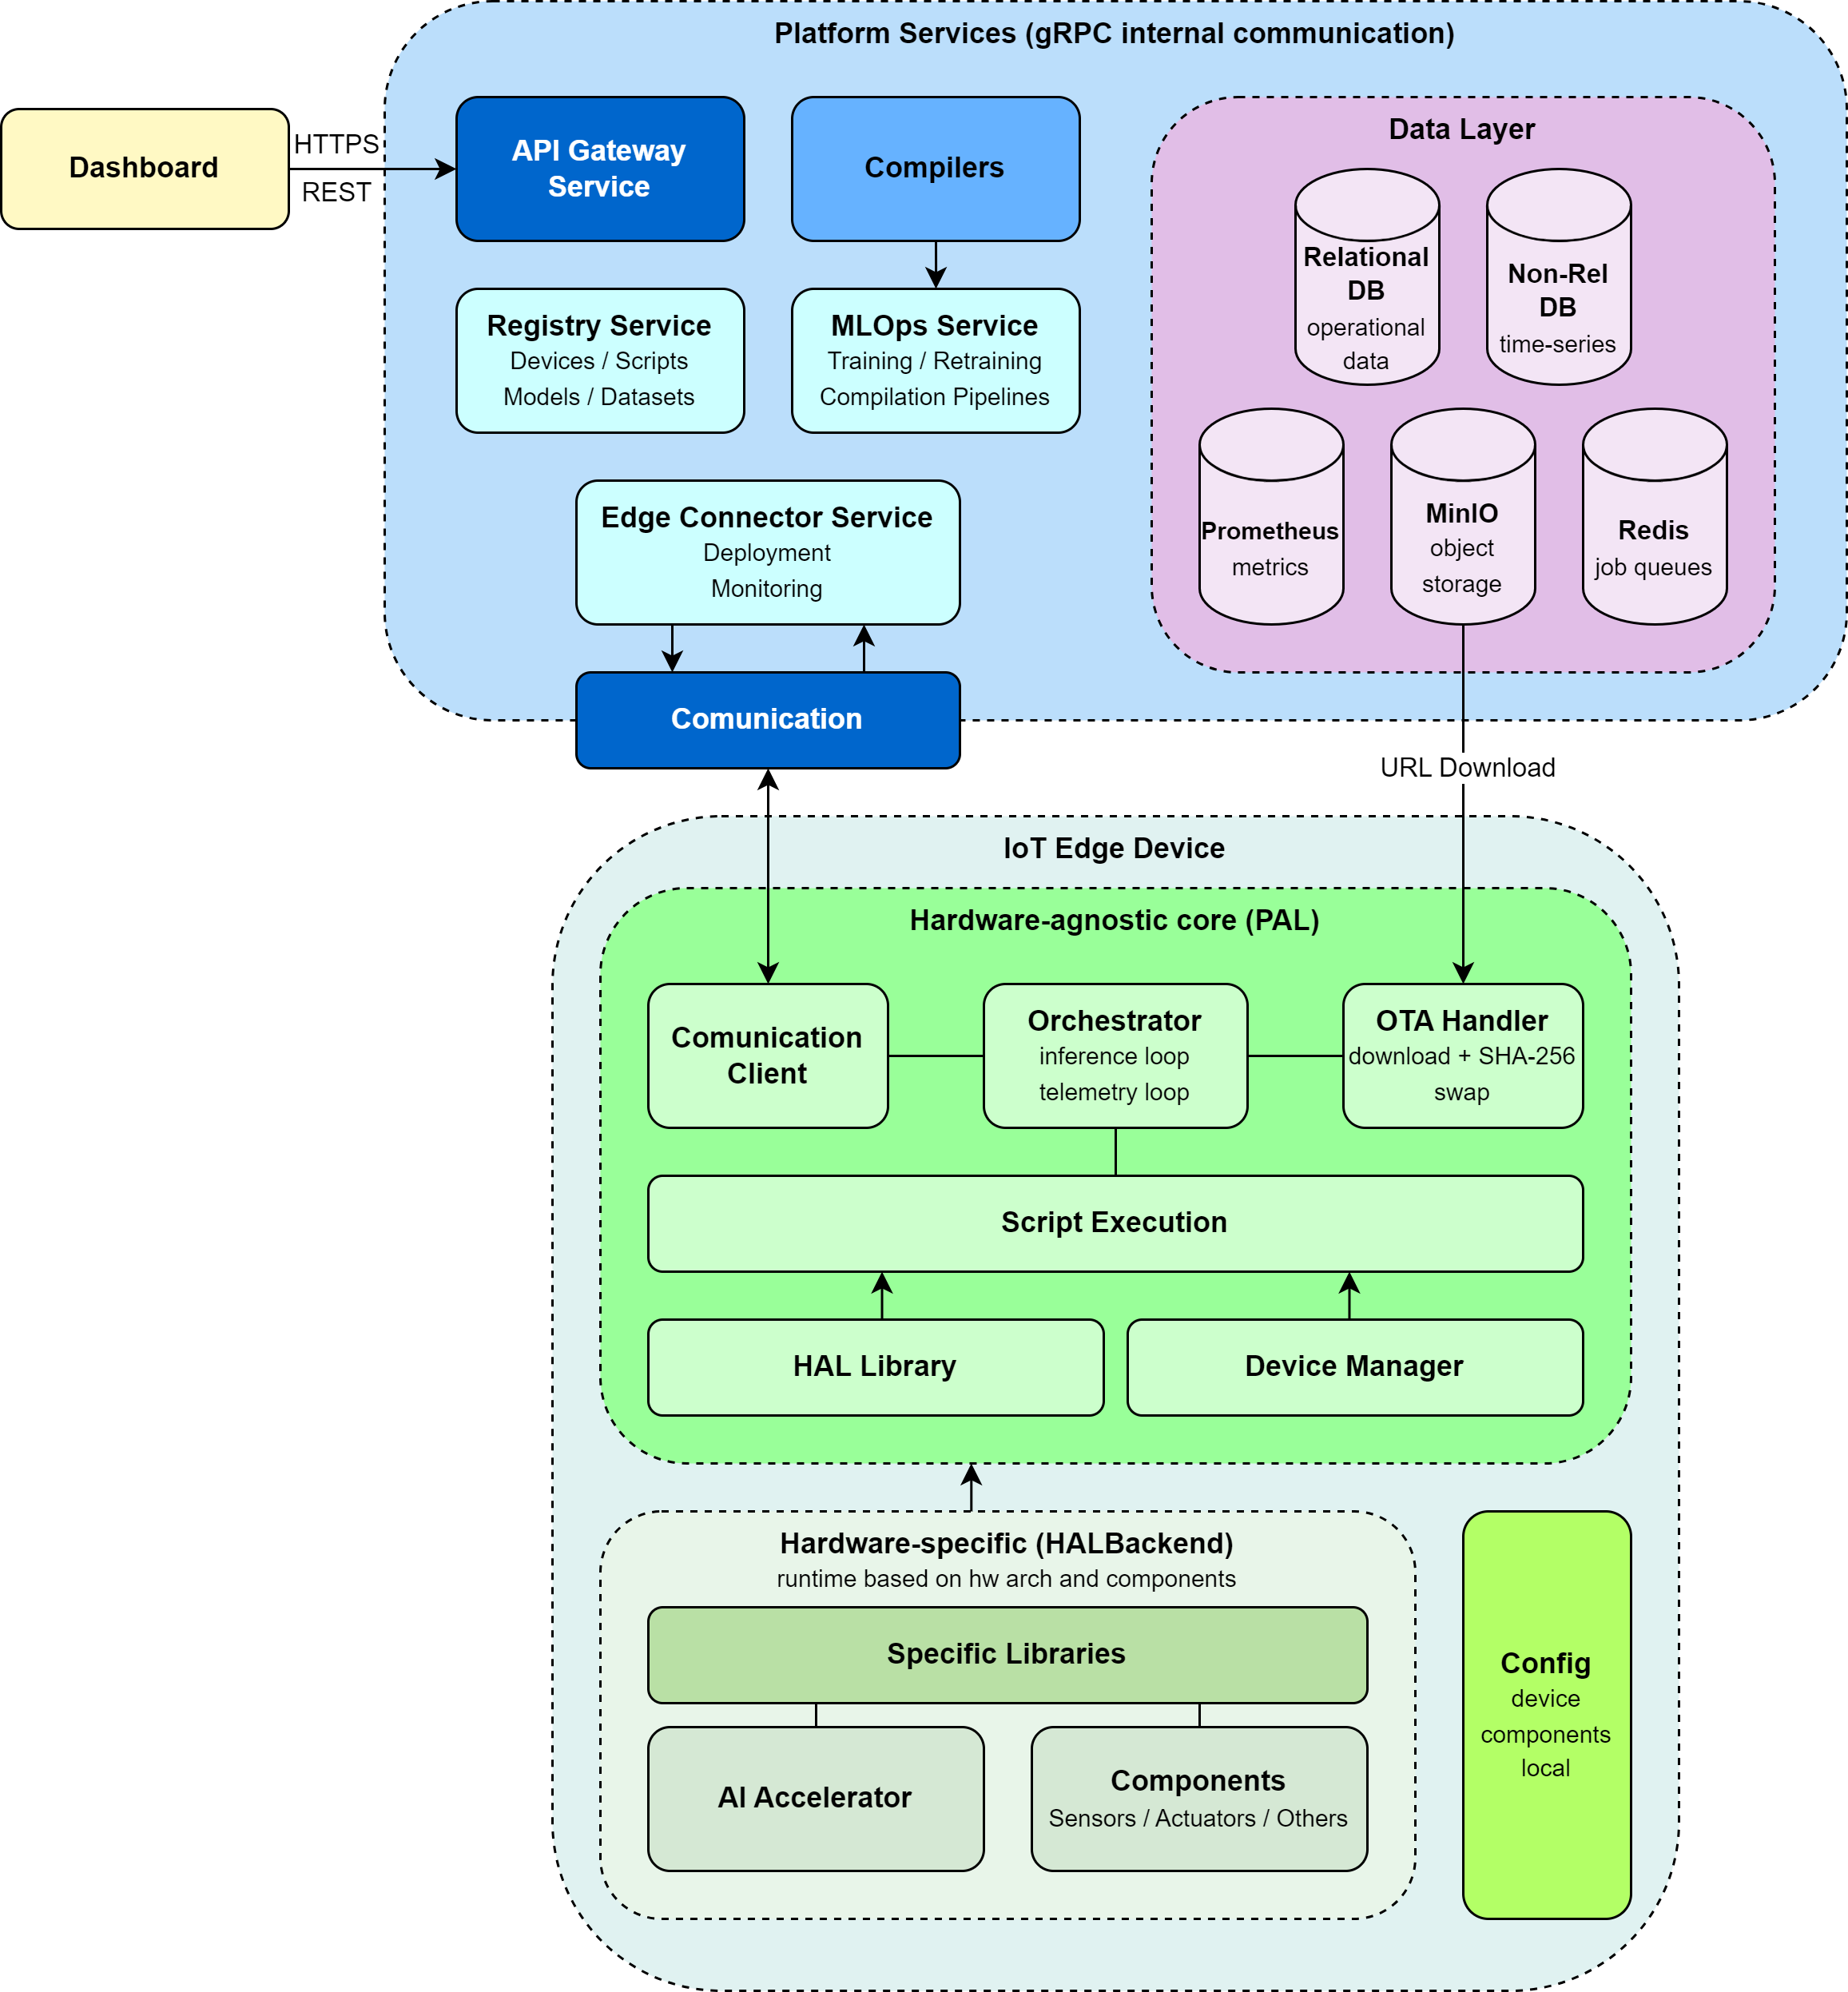
\includegraphics[width=1\linewidth]{images/System Design.png}
    \caption{System Design of the \acrshort{AURA} Platform}
    \label{fig:system_design}
\end{figure}

\subsubsection{User Interface}

The User Interface is a web-based administration dashboard that serves as the centralized interface for platform operators. It provides complete functional control over registered devices, custom scripts, and the lifecycle of \gls{ML} models. Through this dashboard, users can perform the following key tasks:
\begin{itemize}
    \item \textbf{Device Inventory and Management}: Register new target hardware, declare and configure attached sensors and actuators, and track active statuses and connection history.
    \item \textbf{Model Repository, Training and Retraining}: Upload trained neural network weight templates, configure dataset packages, and initiate and track training or fine-tuning epochs with real-time log streaming.
    \item \textbf{Script Registry}: Manage preprocessing and postprocessing Python scripts that wrap model inferences to manipulate input/output data.
    \item \textbf{Deployment Orchestration}: Configure and trigger single-click deployment orders that link a target device with a compiled model and its companion execution script.
    \item \textbf{Live Telemetry and Monitoring}: Visualize time-series hardware usage (e.g., \gls{CPU} percentage, \gls{RAM} footprint) and parse inference outputs streamed in real time from field deployments.
\end{itemize}

\subsubsection{Cloud/Server Platform}\label{sec:proposal:design:cloud}

The Cloud/Server Platform is the central orchestration and management backend of the system. It is structured as a collection of decoupled, specialized services that coordinate internally using secure, low-latency communication interfaces. The platform is divided into two primary layers: the \textbf{Service Layer} and the \textbf{Data Layer}.

\begin{itemize}
    
    \item \textbf{Service Layer}: This layer divides platform tasks across four micro-services described in \autoref{tab:microservices}.

    \begin{table}[H]
        \centering
        \caption{Micro-Services of the \acrshort{AURA} Cloud/Server Platform}
        \label{tab:microservices}
        \begin{tabular}{p{0.2\textwidth}p{0.75\textwidth}}
            \hline
            \textbf{Service} & \textbf{Description} \\
            \hline
            \textbf{\gls{API} Gateway} &
                Exposes the external entry point for user interaction, validating user credentials and routing commands to the appropriate internal services. It also manages large binary file uploads directly to storage buckets to avoid bottlenecking. \\
            \textbf{Registry Service} &
                Serves as the central administrative ledger. Manages database entities using a unified relational schema to persist details of registered edge nodes, datasets, \gls{ML} model definitions, custom scripts, and deployment configurations. \\
            \textbf{\gls{MLOps} Service} &
                Operates as a decoupled asynchronous job executor. Executes model training/retraning, and executes hardware-specific compiler suites to optimize models for targets. Uses queued background workers to process heavy workloads without blocking \gls{API} responsiveness. \\
            \textbf{Edge Connector Service} &
                Handles bidirectional edge communication. Manages deployment of \gls{AI} models and listens to telemetry streams and inference outputs from field devices. \\
            \hline
        \end{tabular}
    \end{table}

    \item \textbf{Data Layer}: The platform relies on specialized, distinct storage mechanisms to handle the diverse data requirements of the system as shown in \autoref{tab:storages}

        \begin{table}[H]
        \centering
        \caption{Storages of the \acrshort{AURA} Cloud/Server Platform}
        \label{tab:storages}
        \begin{tabular}{p{0.2\textwidth}p{0.75\textwidth}}
            \hline
            \textbf{Service} & \textbf{Description} \\
            \hline
            \textbf{Relational Storage} &
                Manages structural metadata for devices, model registrations, dataset records, scripts, and deployments, ensuring transactional consistency. \\
            \textbf{Non-Relational Storage} &
                Records high-frequency telemetry histories and \gls{AI} inference results. \\
            \textbf{Object Storage (MinIO)} &
                Stores raw training datasets, original model weight files, custom execution scripts, and compiled target-specific model binaries. \\
            \textbf{Message Queue / Cache (Redis)} &
                Manages task coordination for background training and compilation jobs, handles model training log streaming, and manages real-time status flags. \\
            \textbf{Metrics Engine (Prometheus)} &
                Aggregates and stores real-time system performance and device telemetry metrics (e.g. \gls{CPU}/\gls{RAM} usage levels), enabling long-term monitoring and alerting. \\
            \hline
        \end{tabular}
    \end{table}
    
\end{itemize}

\subsubsection{\texorpdfstring{\acrshort{IoT}}{IoT} Edge Devices}

Each physical \gls{IoT} edge device runs an embedded runtime instance that processes inference tasks directly at the edge. The runtime is designed around a \textbf{\gls{PAL}} that isolates execution logic from hardware specifics, using dedicated backends to interact with diverse hardware acceleration targets.

\begin{itemize}
    \item \textbf{Hardware-Agnostic Core (\gls{PAL})}:
    \begin{itemize}
        \item \textbf{Orchestrator}: Coordinates the execution of local inference pipelines, retrieves hardware health metrics, and sends regular status and telemetry updates to the cloud platform.
        \item \textbf{\gls{OTA} Handler}: Listens for deployment commands from the cloud platform, downloads updated models and script files, verifies their integrity, and reloads the inference engine.
        \item \textbf{Execution Scripts}: The runtime executes a unified processing pipeline that wraps the hardware inference model. This script contains custom preprocessing logic (e.g., to crop input frames from cameras/sensors) and custom postprocessing logic (e.g., to threshold bounding boxes and classes) before the telemetry and inference results are published.
    \end{itemize}

    \item \textbf{Hardware-Specific Layer (\acrshort{HAL}Backend)}: Target-specific backends wrap native compiler runtime libraries, translating the generic inference requests from the Orchestrator into optimized, hardware-accelerated execution instructions.
\end{itemize}